\newpage
\section{Introduction}
\subsection{Sections planes}
\subsubsection{Le cylindre}

Quelles formes peut-on obtenir en coupant un cylindre avec un plan ?

\vspace{1cm}

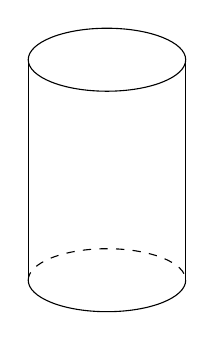
\begin{tikzpicture}[scale = 0.8]
\draw (0,0) ellipse (1.25 and 0.5);
\draw (-1.25,0) -- (-1.25,-3.5);
\draw (-1.25,-3.5) arc (180:360:1.25 and 0.5);
\draw [dashed] (-1.25,-3.5) arc (180:360:1.25 and -0.5);
\draw (1.25,-3.5) -- (1.25,0);  

\end{tikzpicture}


Et si le cylindre avait une hauteur infinie ?

\subsubsection{Section plane avec une lampe de poche}

À l’aide d’un carton et d’une lampe de poche, créez différentes formes en deux dimensions sur le carton.
\begin{enumerate}
    \item Combien de formes différentes pouvez-vous obtenir ? Dessinez-les.
    \item Quelle est la forme tridimensionnelle du faisceau lumineux émis par la lampe de poche ?
    \item Quels éléments influencent la forme obtenue sur le carton ?
\end{enumerate}

\newpage
\subsubsection{Le cône}\label{section:coneplan}

\begin{figure}[!htb]
    \centering 
    
    \caption[Section de cône]{Les coniques propres comme sections de cône \raisebox{-.2ex}{
\includegraphics[height=4ex]{./images/icon/roue.PNG}} \footnotemark }
    \vspace{0.5cm}
    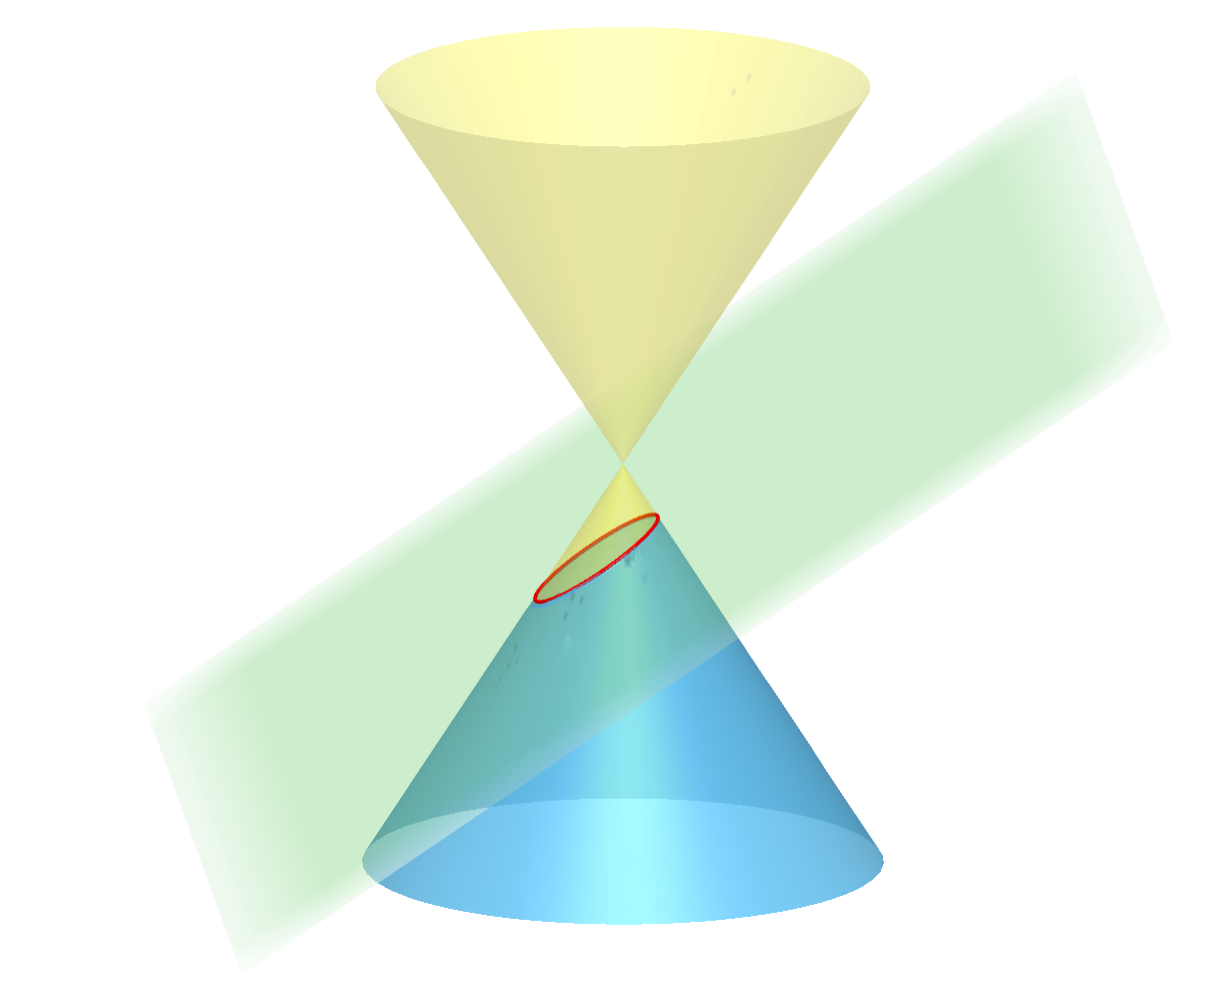
\includegraphics[height=5cm]{./images/3d/cone_ellipse.PNG}
    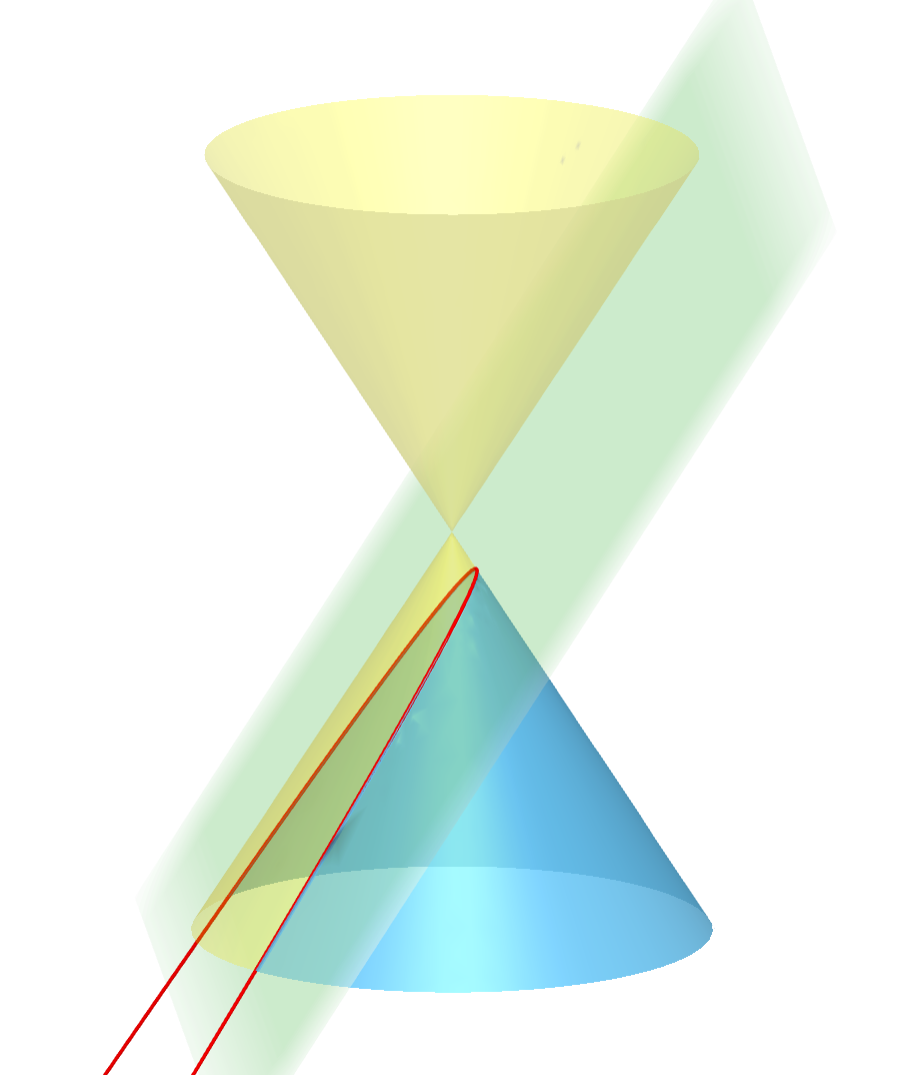
\includegraphics[height=5.4cm]{./images/3d/cone_parabole.PNG}
    \hspace{0.5cm}
    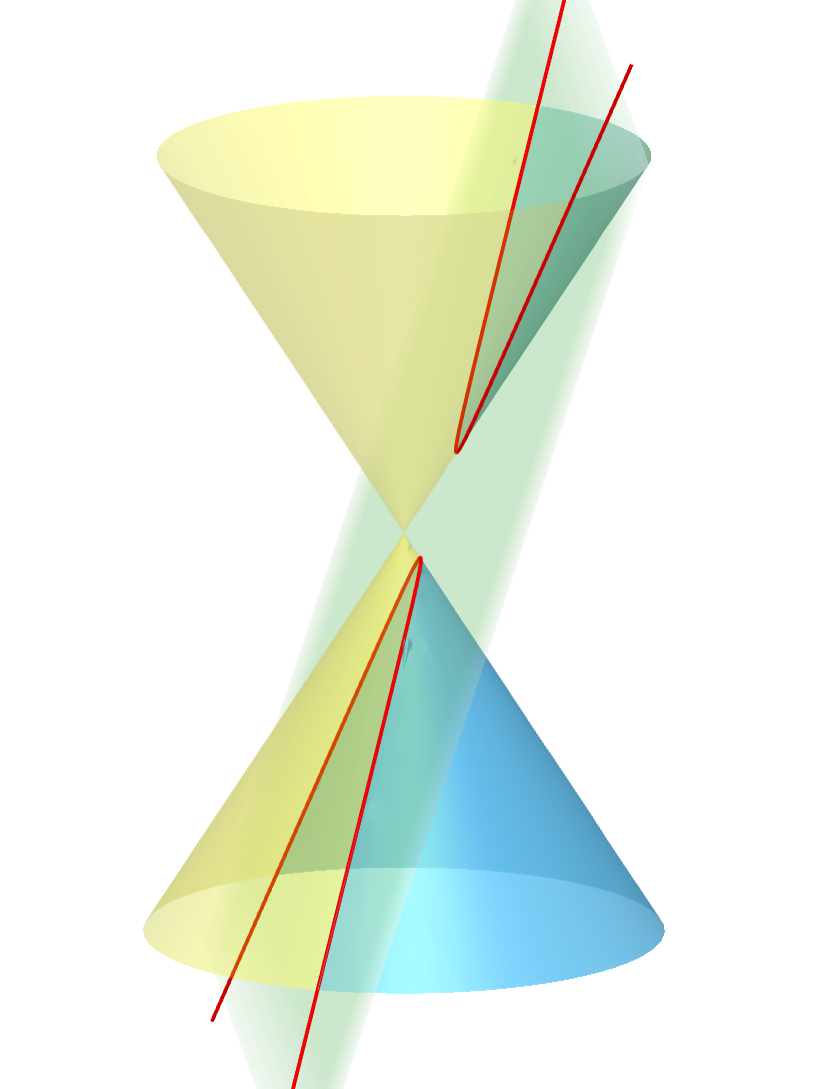
\includegraphics[height=5.4cm]{./images/3d/cone_hyperbole.PNG}
    \label{fig:cone_sections}


\end{figure}
\vspace{7cm}
\begin{figure}[!htb]
    \centering 
    
    \caption[Section de cône]{Les coniques dégénérées comme sections de cône }
    \vspace{0.5cm}
    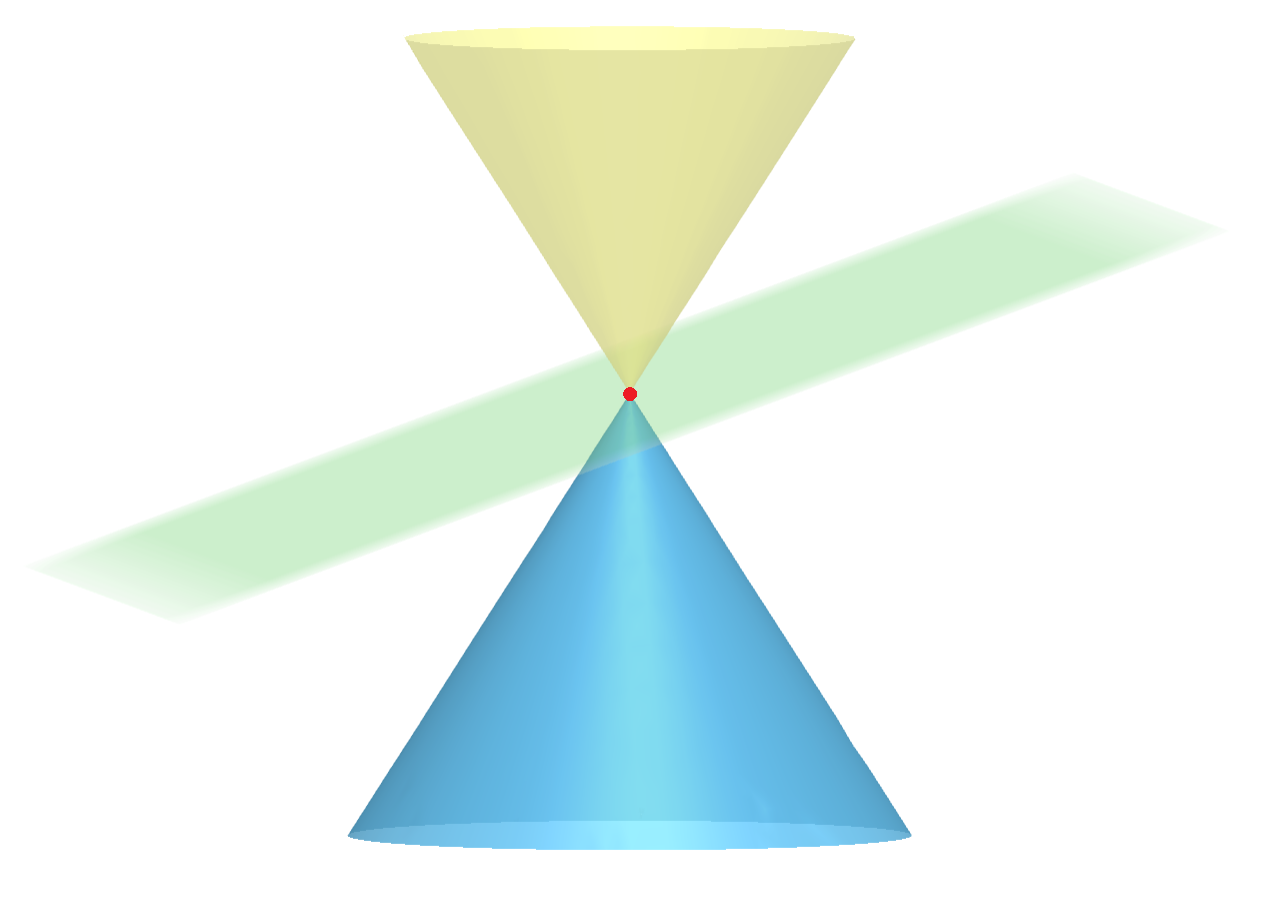
\includegraphics[height=5cm]{./images/3d/cone_point_1.PNG}
    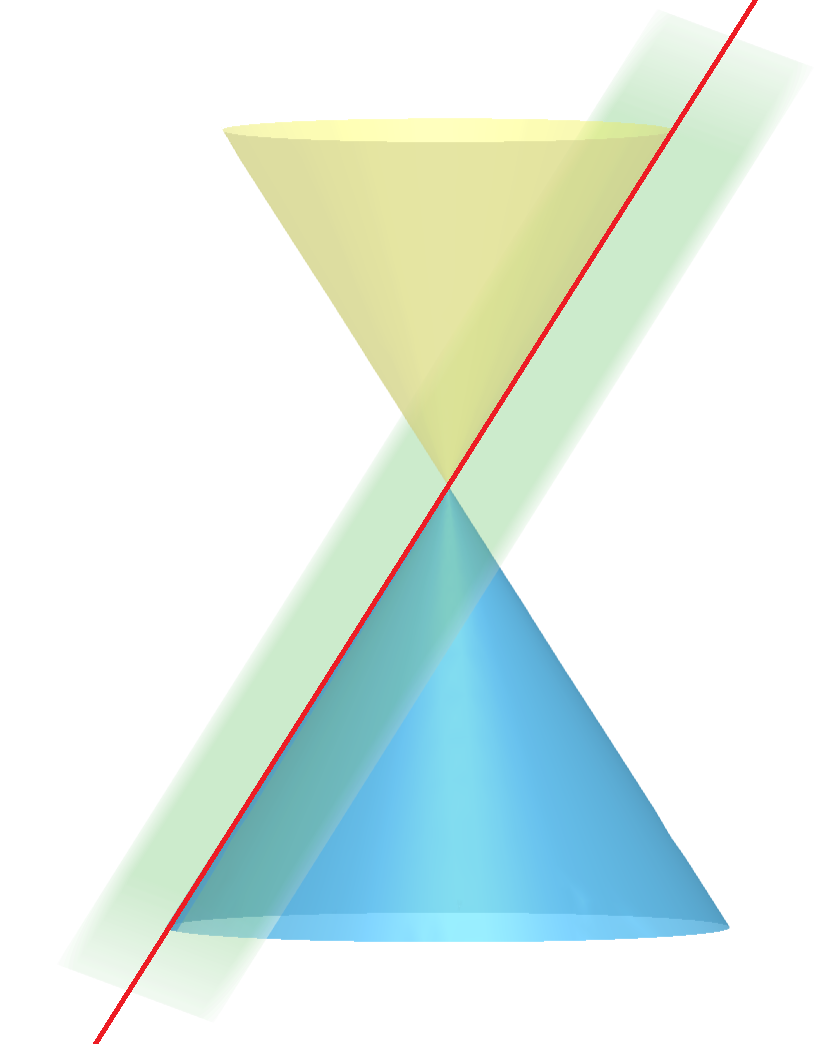
\includegraphics[height=5.20cm]{./images/3d/cone_droite_1.PNG}
        \hspace{1cm}
    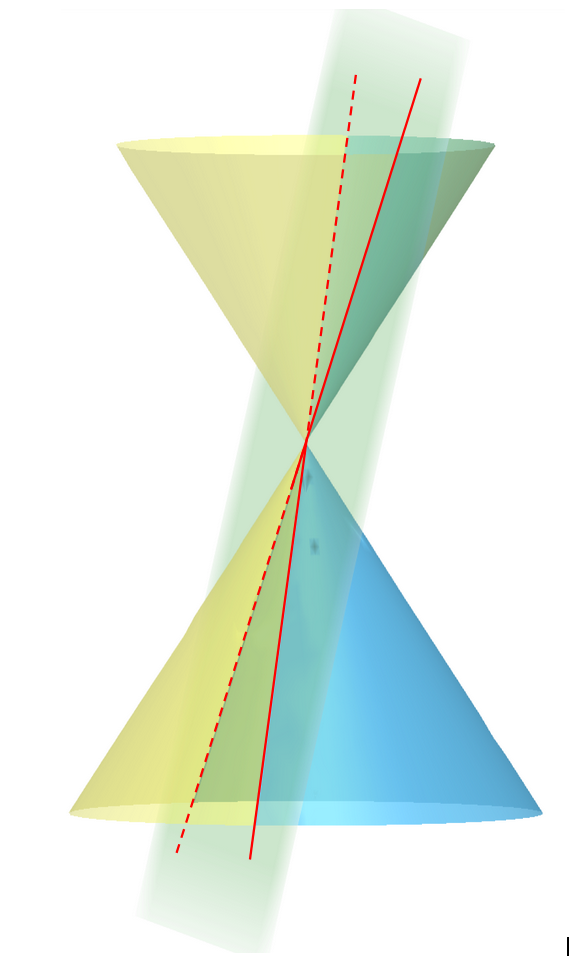
\includegraphics[height=5.7cm]{./images/3d/cone_2droites_1.PNG}
    \label{fig:cone_sections_deg}


\end{figure}
\footnotetext{Jacques Marot, \url{https://www.geogebra.org/classic/dt4yx9xv}}

\newpage
\subsection{Qu'est-ce qu'elles ont de spécial, les coniques ?}
\subsubsection{De Kepler à Newton - le problème à deux corps}
Le problème à deux corps consiste à déterminer le mouvement de deux masses en interaction mutuelle.
En utilisant la loi de la gravitation universelle de Newton, il est possible de décrire analytiquement les trajectoires des deux corps soumis à leur attraction gravitationnelle.
La résolution de ce problème montre que ces trajectoires sont des coniques (ellipses, paraboles ou hyperboles) et qu’elles vérifient les lois de Kepler.
\vfill
Orbite elliptique de Sedna \raisebox{-.7ex}{
\includegraphics[height=4ex]{./images/icon/video.PNG}} \footnote[1]{NASA, \url{https://science.nasa.gov/photojournal/sedna-orbit-animation/}}
\begin{figure}[!ht]
    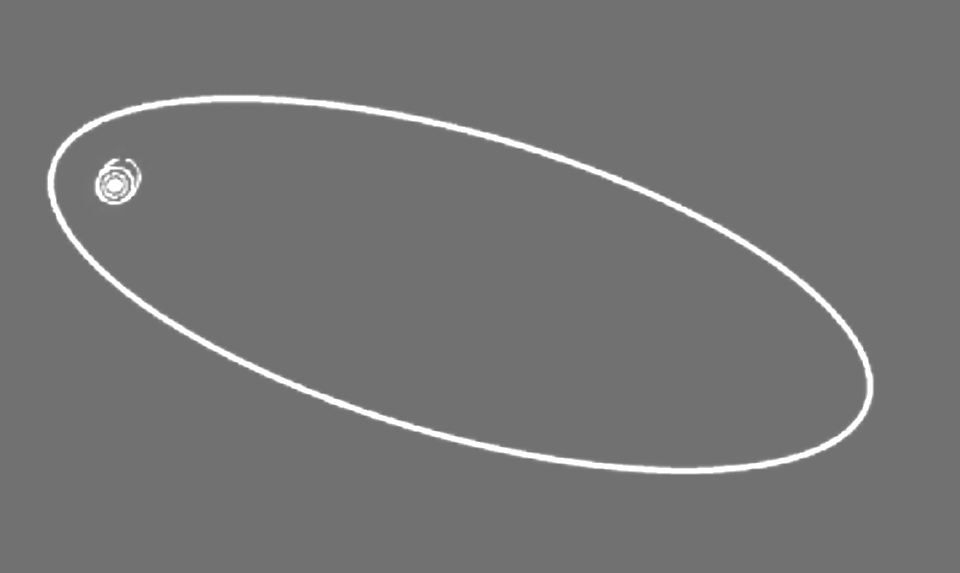
\includegraphics[width = 5cm]{./images/applications/sedna_nb.PNG}
\end{figure}

Orbite hyperbolique de la comète C/2012 S1 (ISON) \raisebox{-.7ex}{
\includegraphics[height=4ex]{./images/icon/video.PNG}} \footnote{NASA, \url{www.youtube.com/watch?v=40wICUY5VmU}}
\begin{figure}[!ht]
    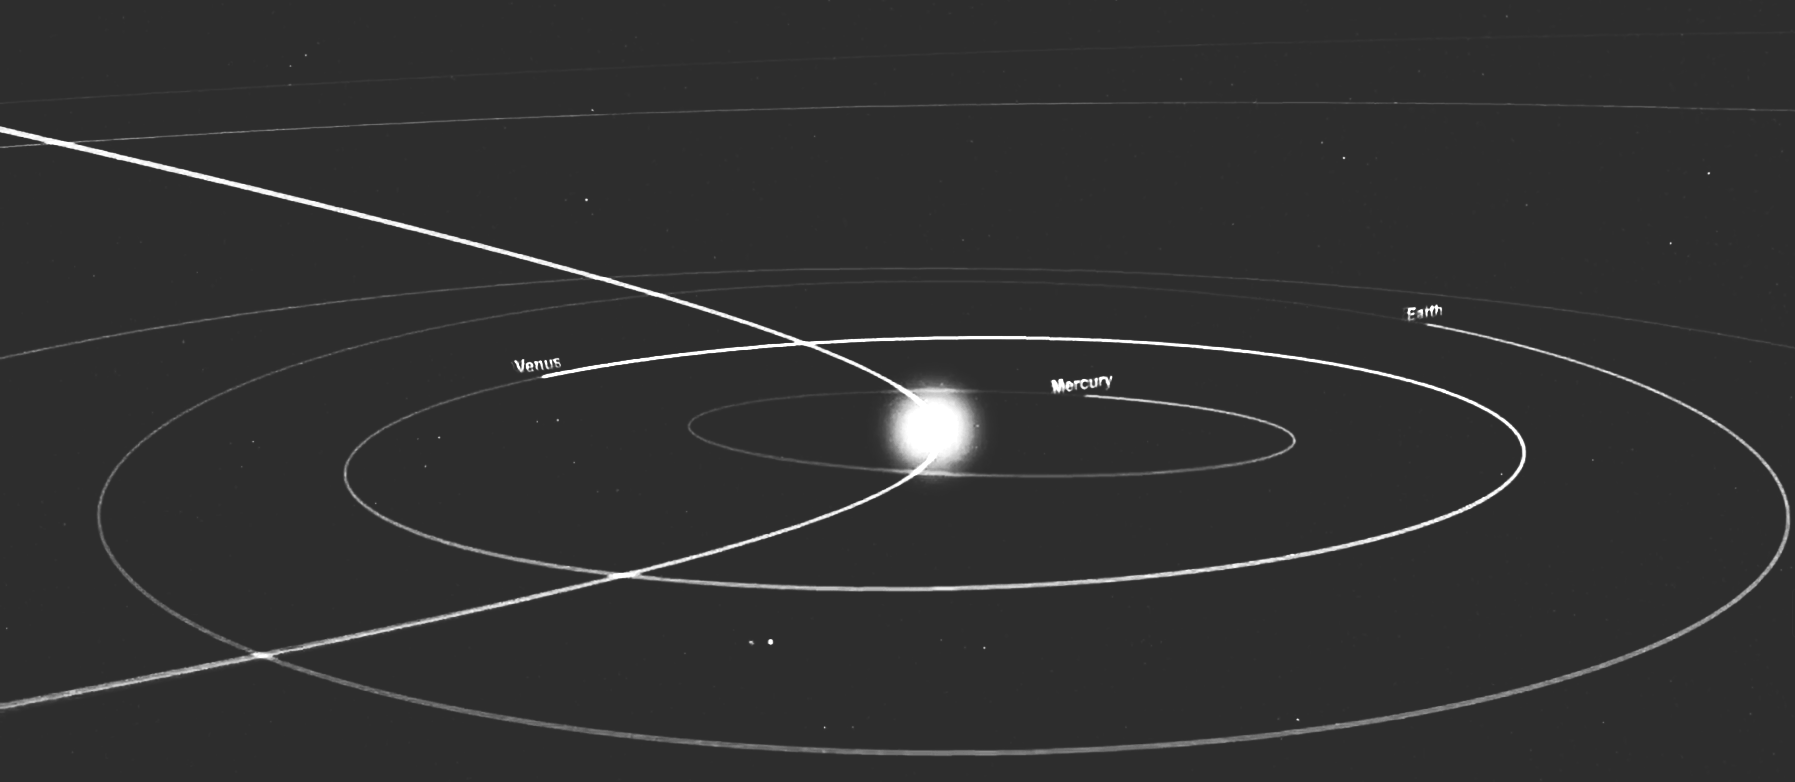
\includegraphics[width = 7cm]{./images/applications/ison_nb.PNG}
\end{figure}

Qu'en est-il du mouvement d'un projectile sur Terre ?

%% IDEA : Ellipse : vitesse de libération faible. MAis donc trajectoire parabolique sur terre ? -> Ellipse en réalité ?
\newpage
\subsubsection{Antennes paraboliques et fours solaires}

\begin{figure}[!ht]
    \begin{subfigure}{0.4\textwidth}
    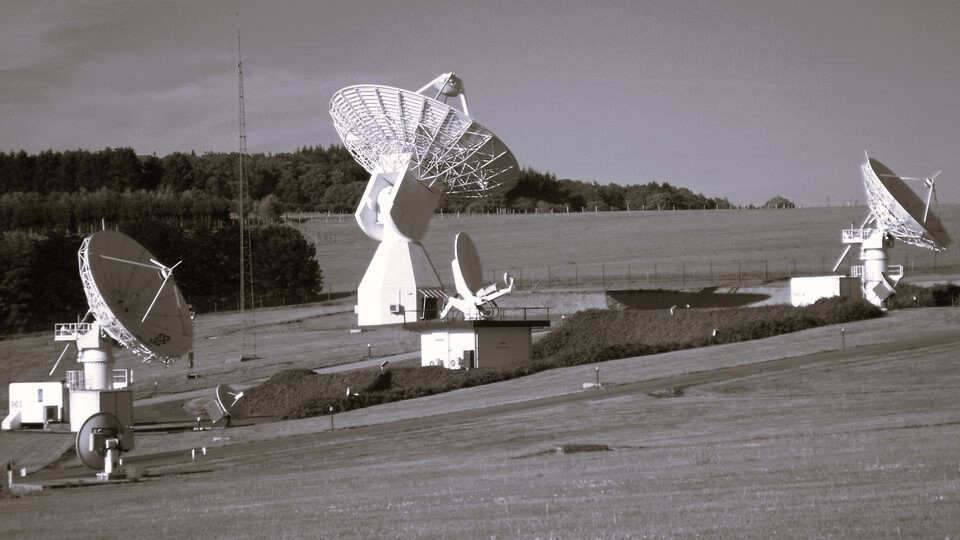
\includegraphics[width=\textwidth]{./images/applications/antenne_redu_nb.jpg}
    \caption[Antennes]{Antennes pour capter les signaux des satellites Galileo\footnotemark[1].}
    \end{subfigure}
\hfill
    \begin{subfigure}{0.4\textwidth}
    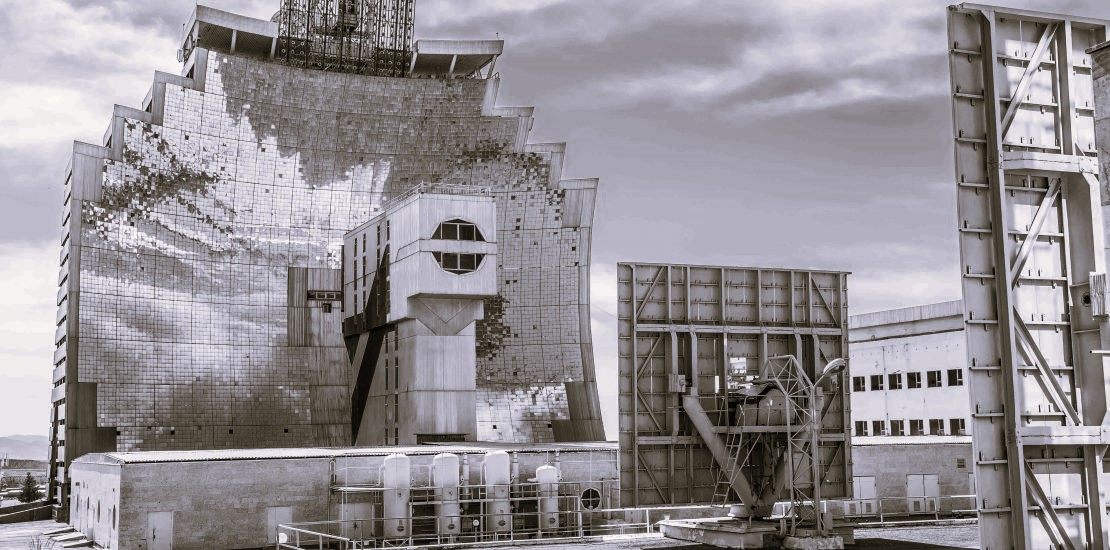
\includegraphics[width=\textwidth]{./images/applications/four_parkent_nb.jpg}
    \caption[Parkent]{Four solaire à Parkent, Ouzbékistan \footnotemark[2].}
    \end{subfigure}
\vspace{1cm}
    \begin{subfigure}{0.3\textwidth}
        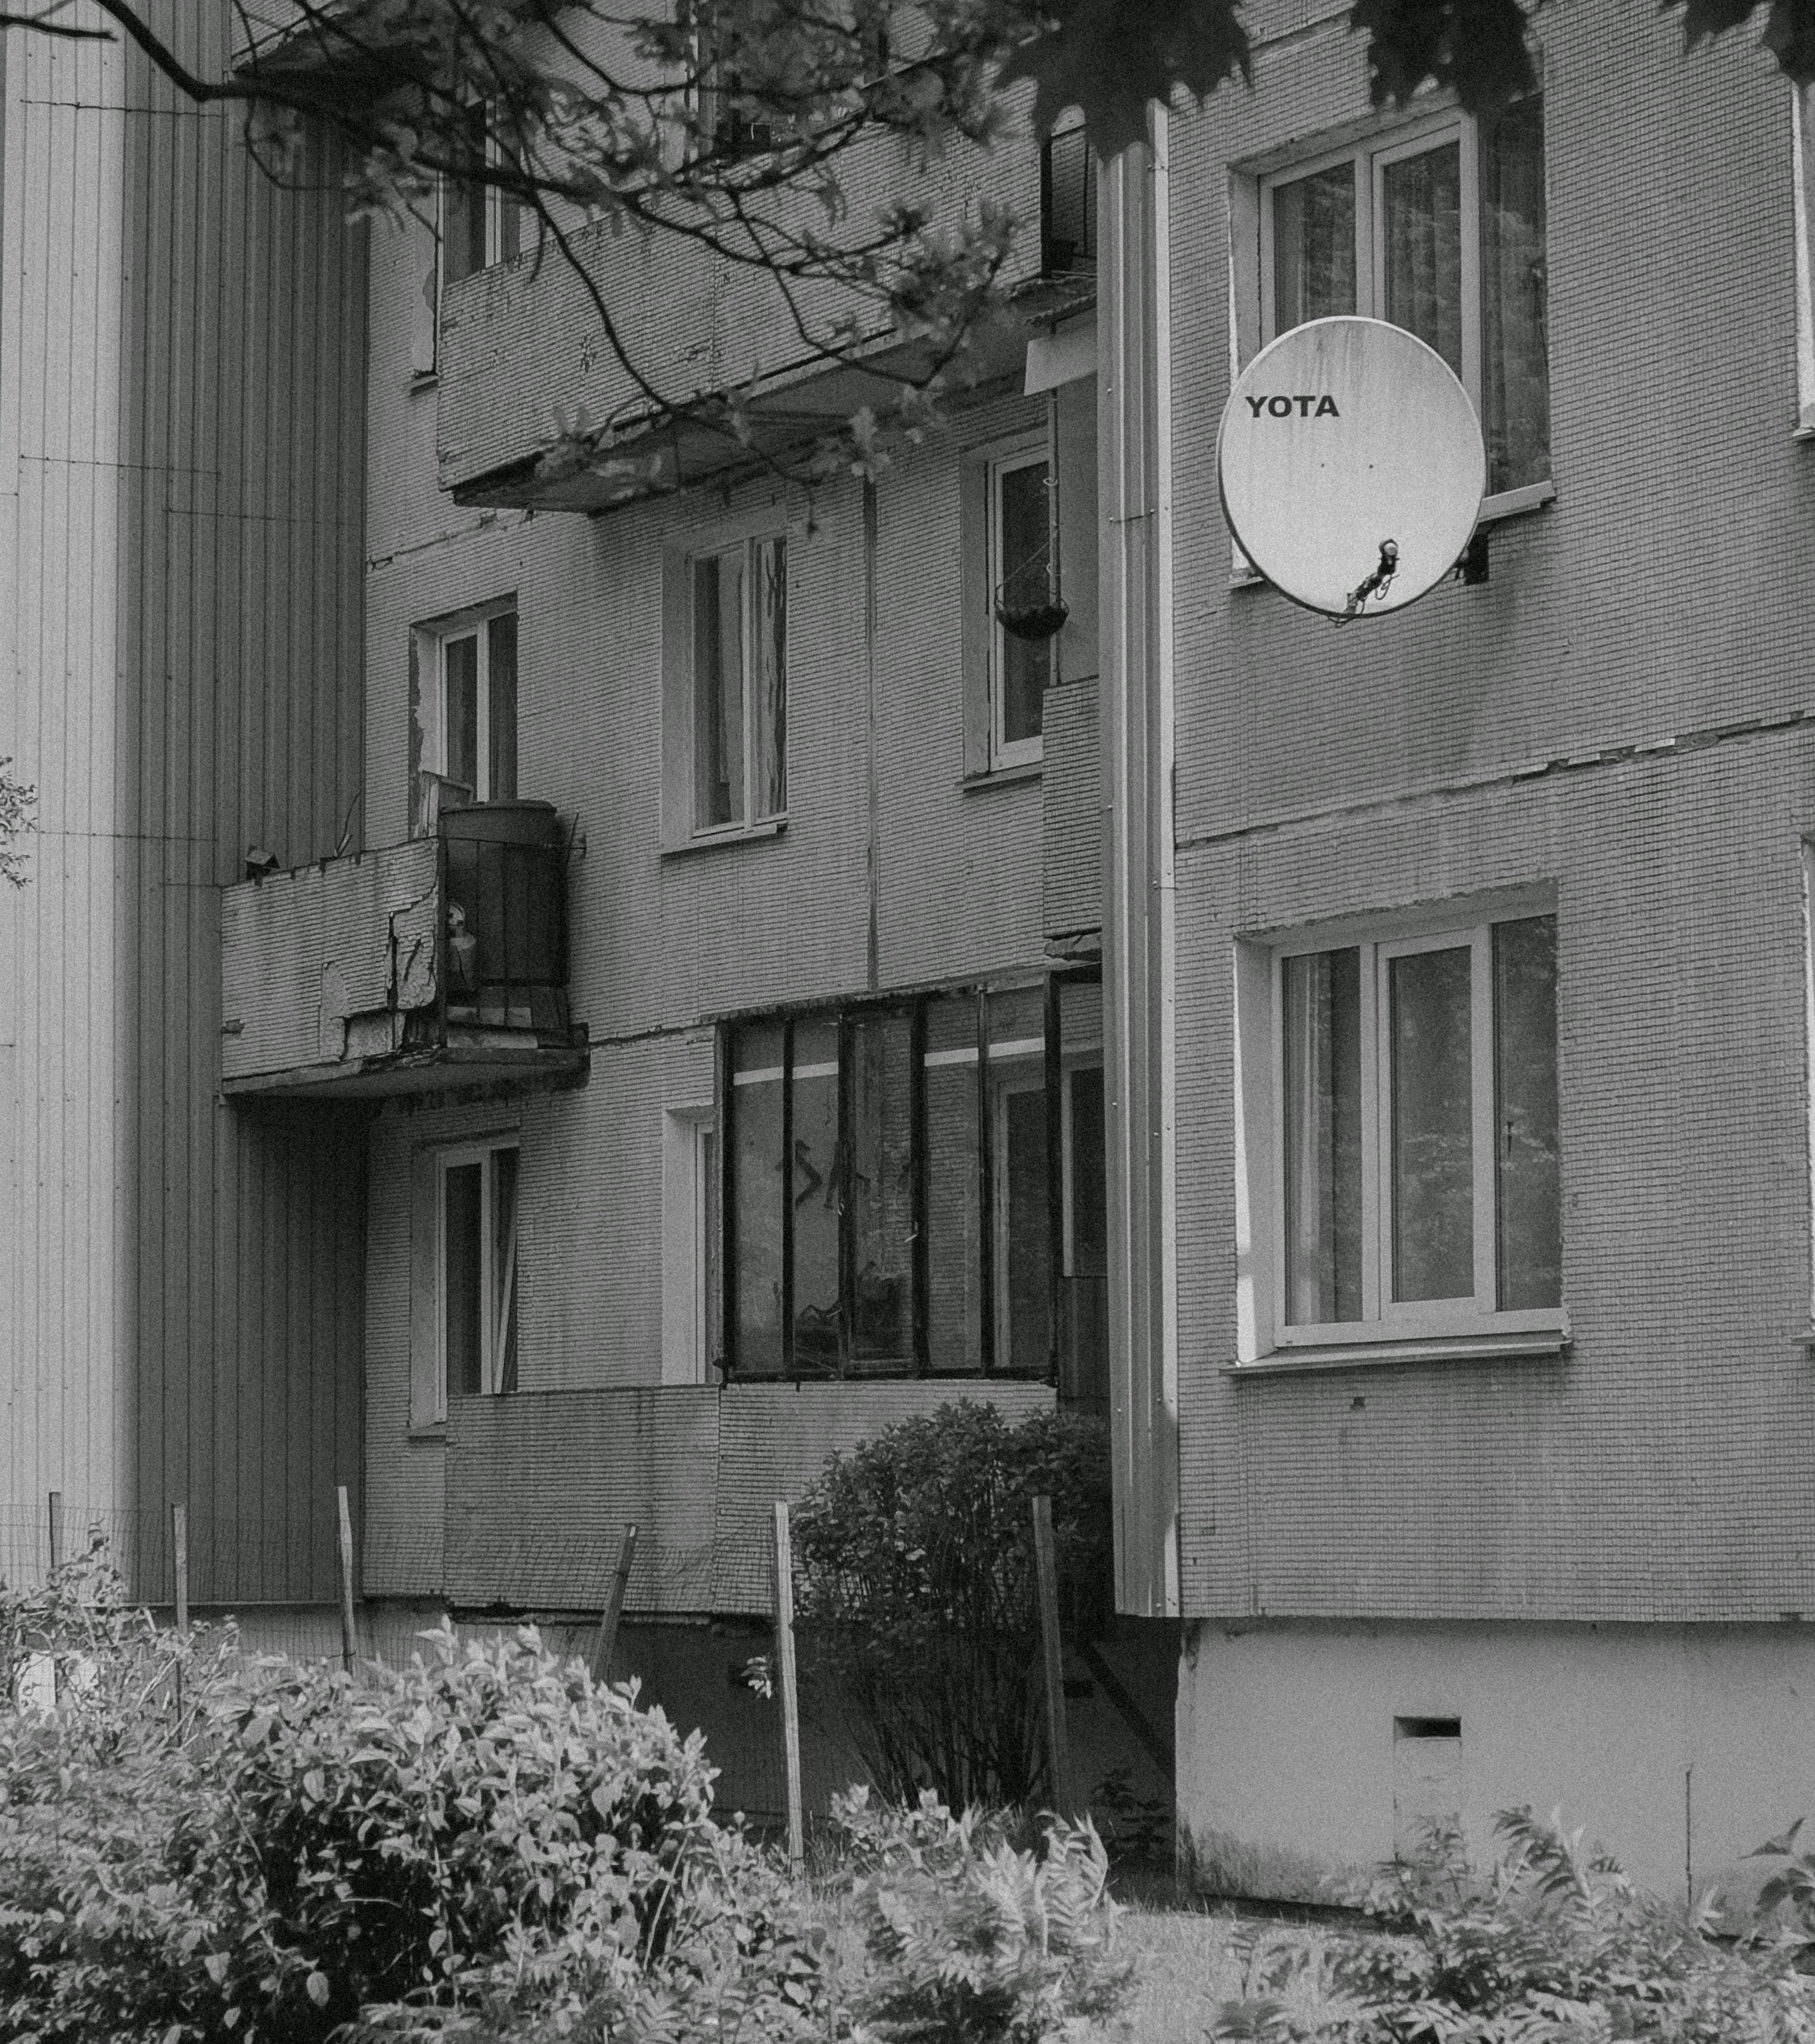
\includegraphics[width=\textwidth]{./images/applications/parabole_tv.jpg}
    \caption[TV]{"Parabole" pour capter les chaînes TV.}
    \end{subfigure}
\hfill
    \begin{subfigure}{0.3\textwidth}
        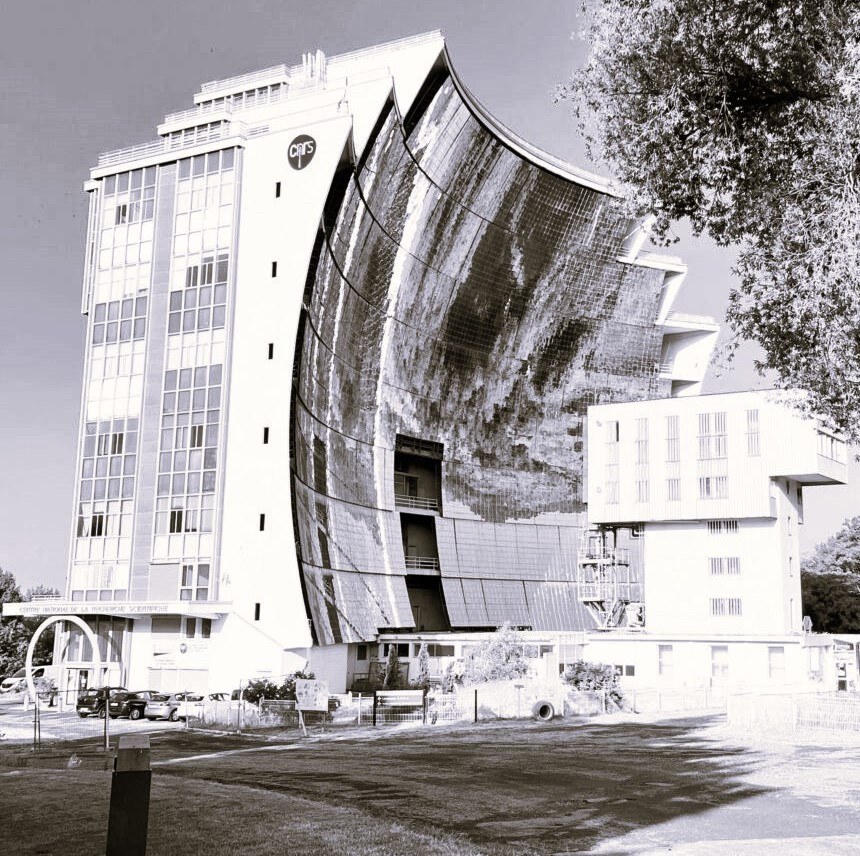
\includegraphics[width=\textwidth]{./images/applications/four_odeillo_nb.jpg}
    \caption[Odeillo]{Four solaire à Odeillo, France\footnotemark[3].}
    \end{subfigure}
\vspace{1cm}
    \begin{subfigure}{0.4\textwidth}
        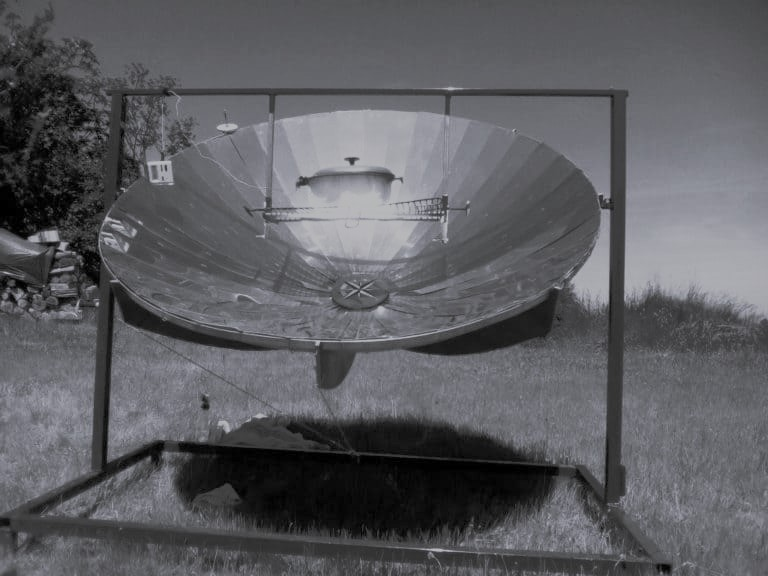
\includegraphics[width=\textwidth]{./images/applications/four_sol_nb.jpg}
    \caption[four]{Four solaire pour cuisiner \footnotemark[4].}
    \end{subfigure}
\end{figure}
\footnotetext[4]{ESA, \url{https://www.esa.int/Space_in_Member_States/Belgium_-_Francais/La_grande_antenne_de_Redu_destinee_aux_satellites_Galileo}}
\footnotetext[5]{Institute of materials science Uzbekistan academy of science, \url{https://imssolar.uz/en/}}
\footnotetext[6]{PROMES CNRS, \url{https://www.promes.cnrs.fr/infrastructures-solaires/fours-solaires-et-systemes-solaires-a-concentration/}}
\footnotetext[7]{Atelier du zephyr, \url{https://atelierduzephyr.org/auto-construction/cuisiner/cuiseur-et-four-solaires/}}

\newpage
\subsubsection{Microscopes et télescopes}
\begin{figure}[!ht]
    \begin{subfigure}{0.4\textwidth}
    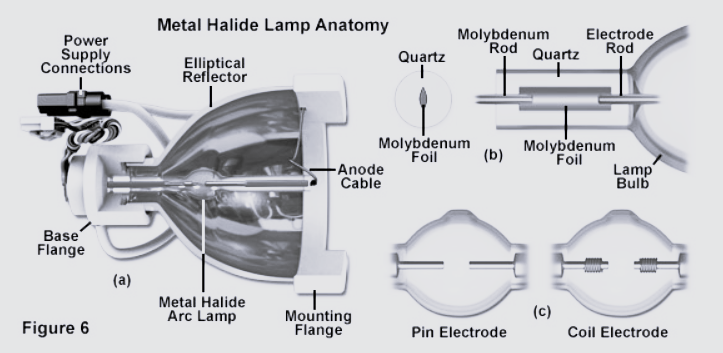
\includegraphics[width=\textwidth]{./images/applications/zeiss_lamp_nb.PNG}
    \caption[Lampe Zeiss]{Lampe aux halogénures métalliques pour microscope à fluorescence \footnotemark[1].}
    \end{subfigure}
\hfill
    \begin{subfigure}{0.4\textwidth}
    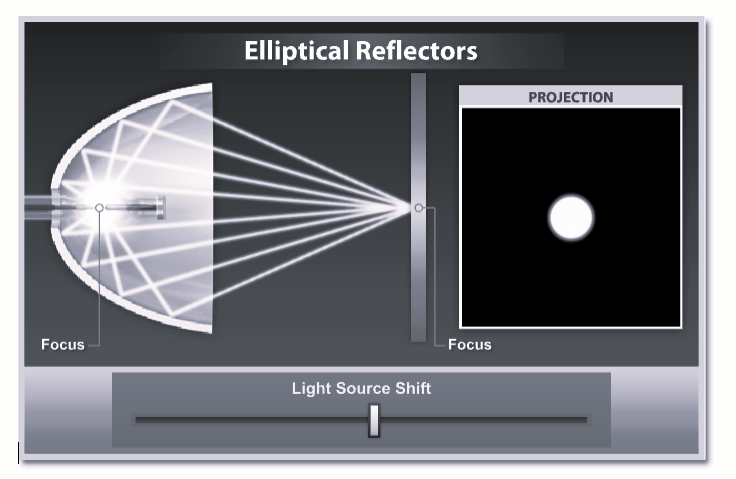
\includegraphics[width=\textwidth]{./images/applications/zeis_1_nb.PNG}
    \caption[Réflecteur elliptique 2]{Réflecteur elliptique dans une lampe pour microscope à fluorescence, source alignée sur un foyer \footnotemark[2]}
    \end{subfigure}
\vspace{1cm}
    \begin{subfigure}{0.4\textwidth}
        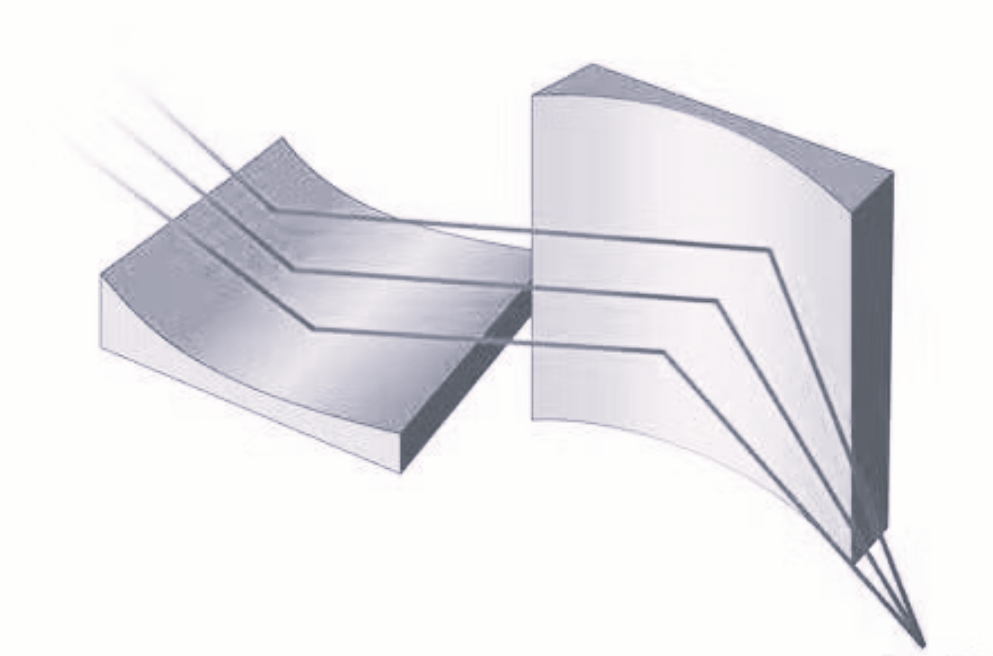
\includegraphics[width=\textwidth]{./images/applications/kbmirror_nb.PNG}
    \caption[KF]{Miroir Kirkpatrick-Baez (KB) \footnotemark[3].}
    \end{subfigure}
\hfill
    \begin{subfigure}{0.4\textwidth}
        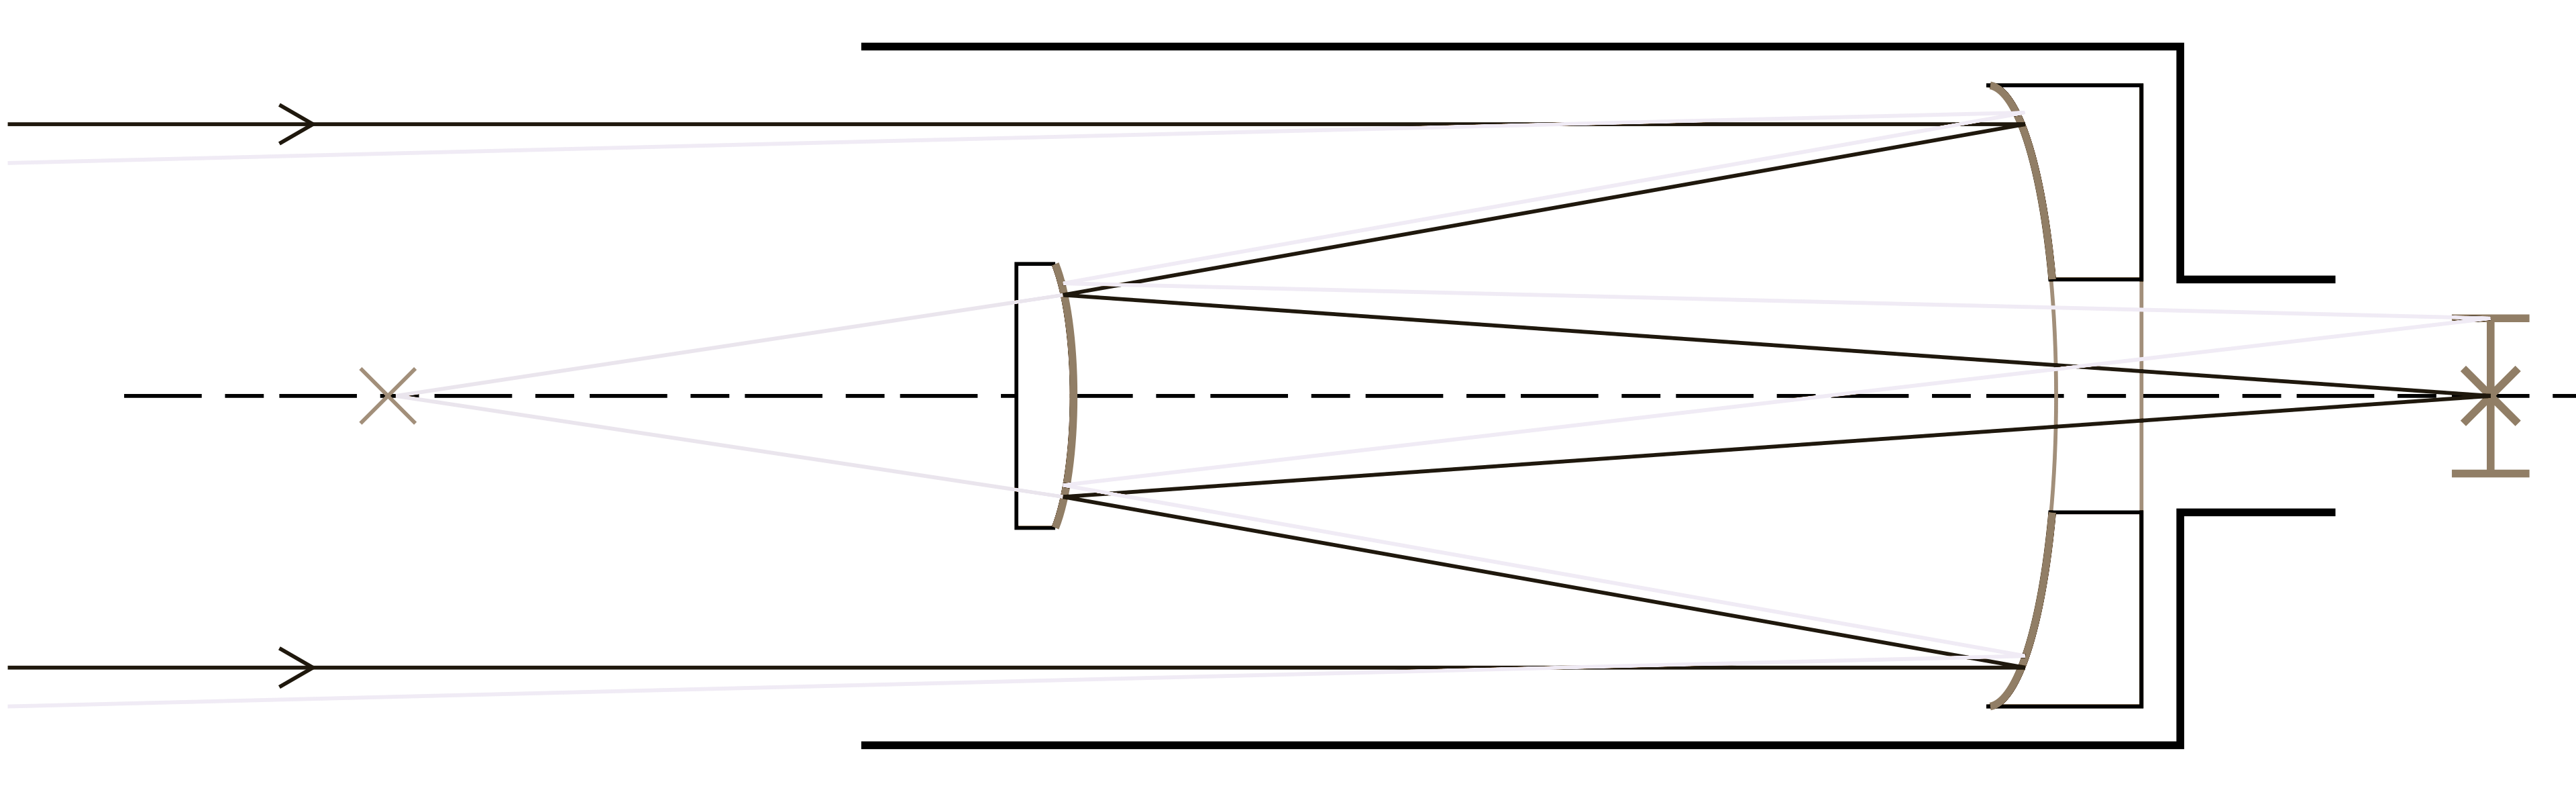
\includegraphics[width=\textwidth]{./images/applications/cassegrain_nb.png}
    \caption[Cassegrain]{Télescope cassegrain avec un miroir hyperbolique et un miroir parabolique \footnotemark[4].}
    \end{subfigure}
\vspace{1cm}
    \begin{subfigure}{0.4\textwidth}
        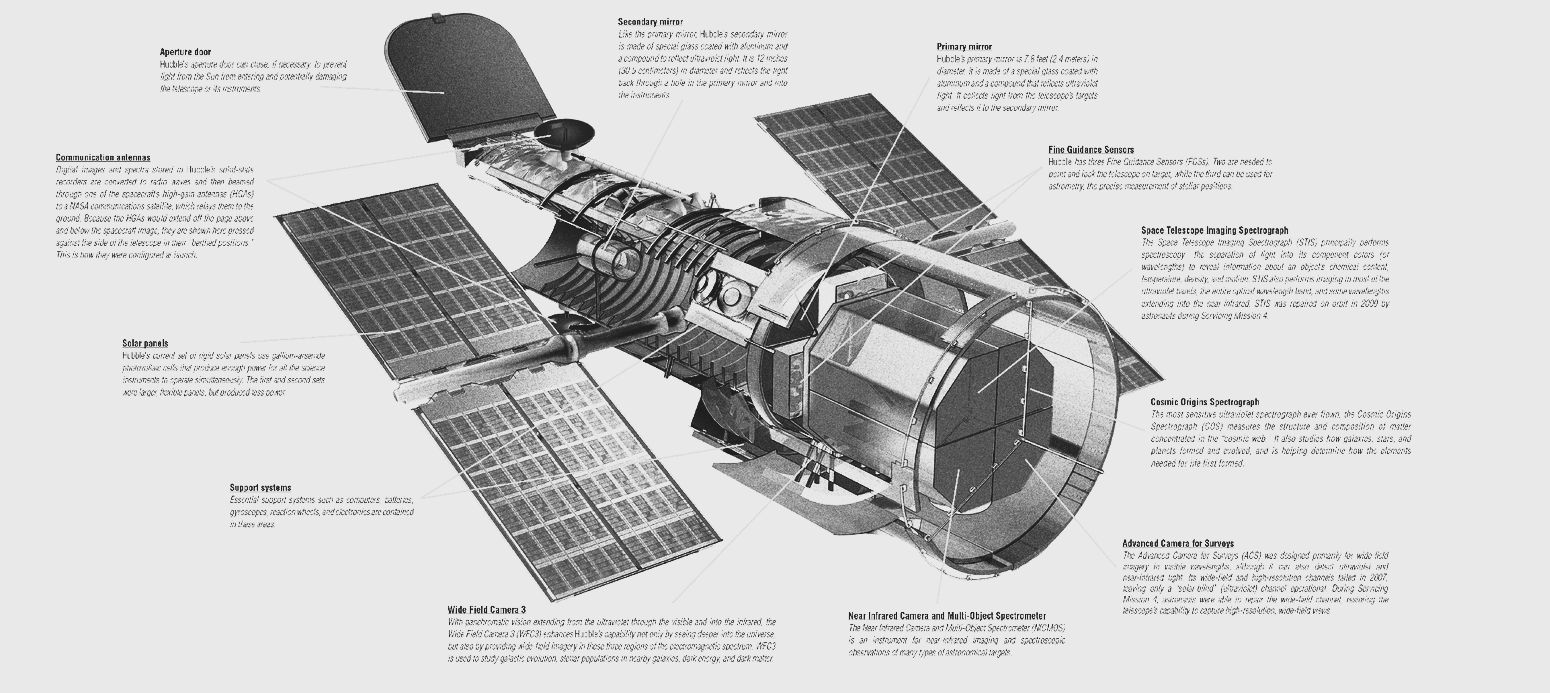
\includegraphics[width=\textwidth]{./images/applications/hubble_design_nb.PNG}
    \caption[Hubble]{Télescope Hubble avec une variante du télescope Cassegrain à 2 miroirs hyperboliques (Ritchey–Chrétien)\footnotemark[5].}
    \end{subfigure}
\end{figure}

\footnotetext[1]{Zeiss, \url{https://zeiss-campus.magnet.fsu.edu/print/lightsources/metalhalide-print.html}}
\footnotetext[2]{Zeiss, \url{https://zeiss-campus.magnet.fsu.edu/tutorials/ellipticalreflectors/indexflash.html}}
\footnotetext[3]{National Accelerator Laboratory, SLAC, Stanford, \url{https://www6.slac.stanford.edu/news/2011-10-11-k-b-mirrors-harness-x-rays-science}}
\footnotetext[4]{Wikipedia, \url{https://en.wikipedia.org/wiki/Cassegrain_reflector#/media/File:Cassegrain_Telescope.svg}}
\footnotetext[5]{NASA, \url{https://ntrs.nasa.gov/citations/19860055868}}
\newpage
\subsubsection{Structures}
\begin{figure}[!htb]

    \begin{subfigure}{0.4\textwidth}
        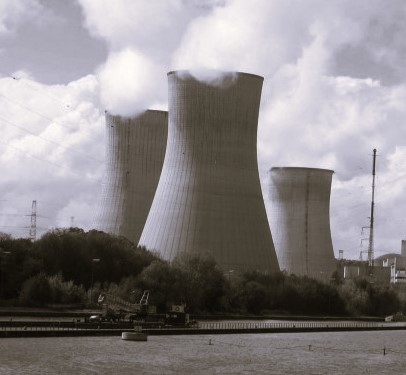
\includegraphics[width=\textwidth]{./images/applications/tihange_nb.jpg}
    \caption[Tihange]{Tours de refroidissement de la centrale électrique de Tihange en forme d'hyperboloïde\footnotemark[1].}
    \end{subfigure}
    \hfill
        \begin{subfigure}{0.5\textwidth}
        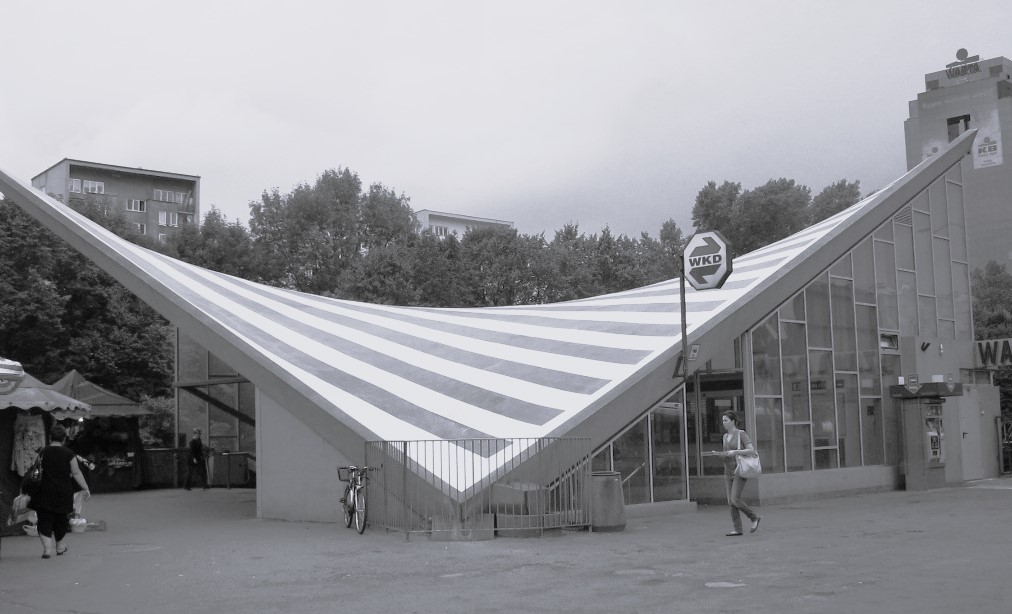
\includegraphics[width=\textwidth]{./images/applications/varsovie_train_nb.jpg}
    \caption[Varsovie]{Gare en forme de paraboloïde hyperbolique à Varsovie \footnotemark[2].}
    \end{subfigure}
\end{figure}

\footnotetext[1]{Engie, \url{https://nuclear.engie-electrabel.be/fr/les-centrales-nucleaires-en-belgique}}
\footnotetext[2]{Wikipedia, \url{https://en.wikipedia.org/wiki/Warszawa_Ochota_railway_station}}

\subsubsection{Généralisation des équations du 2e degré à 2 variables}
Les \textbf{équations du second degré à une inconnue} de la forme
$$ ax^2 + bx + c = d $$
ont été étudiées en 4e secondaire.

En travaillant dans le plan (2D) avec deux variables, les \textbf{équations de droites} ont été abordées :
\[ax + by + c = 0,\]
ainsi qu’une partie des \textbf{équations de paraboles} de la forme
\[
ax^2 + bx + c + dy = 0,
\]
c’est-à-dire celles qui peuvent se réécrire sous la forme d’une \textbf{fonction}
\[
y = ax^2 + bx + c.
\]

En travaillant dans l’espace (3D) avec trois variables, les \textbf{équations de plans} (linéaires) ainsi que leurs intersections ont été étudiées en 5e:
\[
ax + by + cz + d = 0,
\]


Il s’agit maintenant de revenir au plan (2D), tout en faisant des liens avec la 3D, pour étudier les \textbf{équations du second degré à deux variables}, de la forme :
\begin{equation}
    Ax^2 + Bxy + Cy^2 + Dx + Ey + F = 0
\end{equation}
avec \(A, B, C \neq 0\).

Cette équation cartésienne décrit une \textbf{courbe du plan} : il s’agit des \textbf{coniques} (ellipse, parabole, hyperbole).

\subsubsection{Les équations aux dérivées partielles du 2e ordre à 2 variables}
Il est également possible de rencontrer des équations qui décrivent des relations entre des dérivées.

Dans le cas des dérivées partielles du second ordre à deux variables, on obtient une équation de la forme :

\[
A(x,y)\, \dfrac{\partial^2 u}{\partial x^2}
\;+\;
B(x,y)\, \dfrac{\partial^2 u}{\partial x \partial y}
\;+\;
C(x,y)\, \dfrac{\partial^2 u}{\partial y^2}
\;+\;
D(x,y)\, \dfrac{\partial u}{\partial x}
\;+\;
E(x,y)\, \dfrac{\partial u}{\partial y}
\;+\;
F(x,y)\, u
\;=\;
G(x,y).
\]

Le lien avec les coniques est ici algébrique.  
Les équations de cette forme sont également classées en elliptiques, paraboliques ou hyperboliques.

Elles servent à modéliser différents phénomènes physiques, par exemple :
\begin{itemize}
    \item la diffusion de la chaleur (équations paraboliques),
    \item la propagation des ondes (équations hyperboliques),
    \item les situations d’équilibre ou d’état stationnaire (équations elliptiques).
\end{itemize}



